\chapter{Scramble architecture}
\label{ch:Scramble architecture}

Scramble is a tool to realize inter-operability between different MANO frameworks. To achieve this, scramble adds support for translation and splitting of descriptors and provides python wrappers for REST APIs for OSM, SONATA and Pishahang.
\section{Architecture}
\paragraph{}
The services of scramble resides as a plugin within Pishahang MANO framework. In the scope of this project, the plugin has been implemented in Pishahang. The plugin enables cross MANO communication. 

With scramble, hierarchical orchestration is possible. In the figure \ref{fig:scramble-arch}, the high-level architecture of such a scenario is shown. Here, Pishahang instances are installed with the scramble plugin thus enabling it to communicate and manage child MANO instances. Service requests received by the higher level Phishahang MANO instances in the hierarchy can be redirected to lower level MANOs i.e, to either OSM or Pishahang.

\paragraph{}
Scramble is composed of three main services listed below. These are discussed in detail in the following sections.
\begin{itemize}
	\item Translator
	\item Splitter
	\item Wrapper(adaptor)
\end{itemize}


ScrambleArchitecture
\begin{figure}[h]
	\centering
	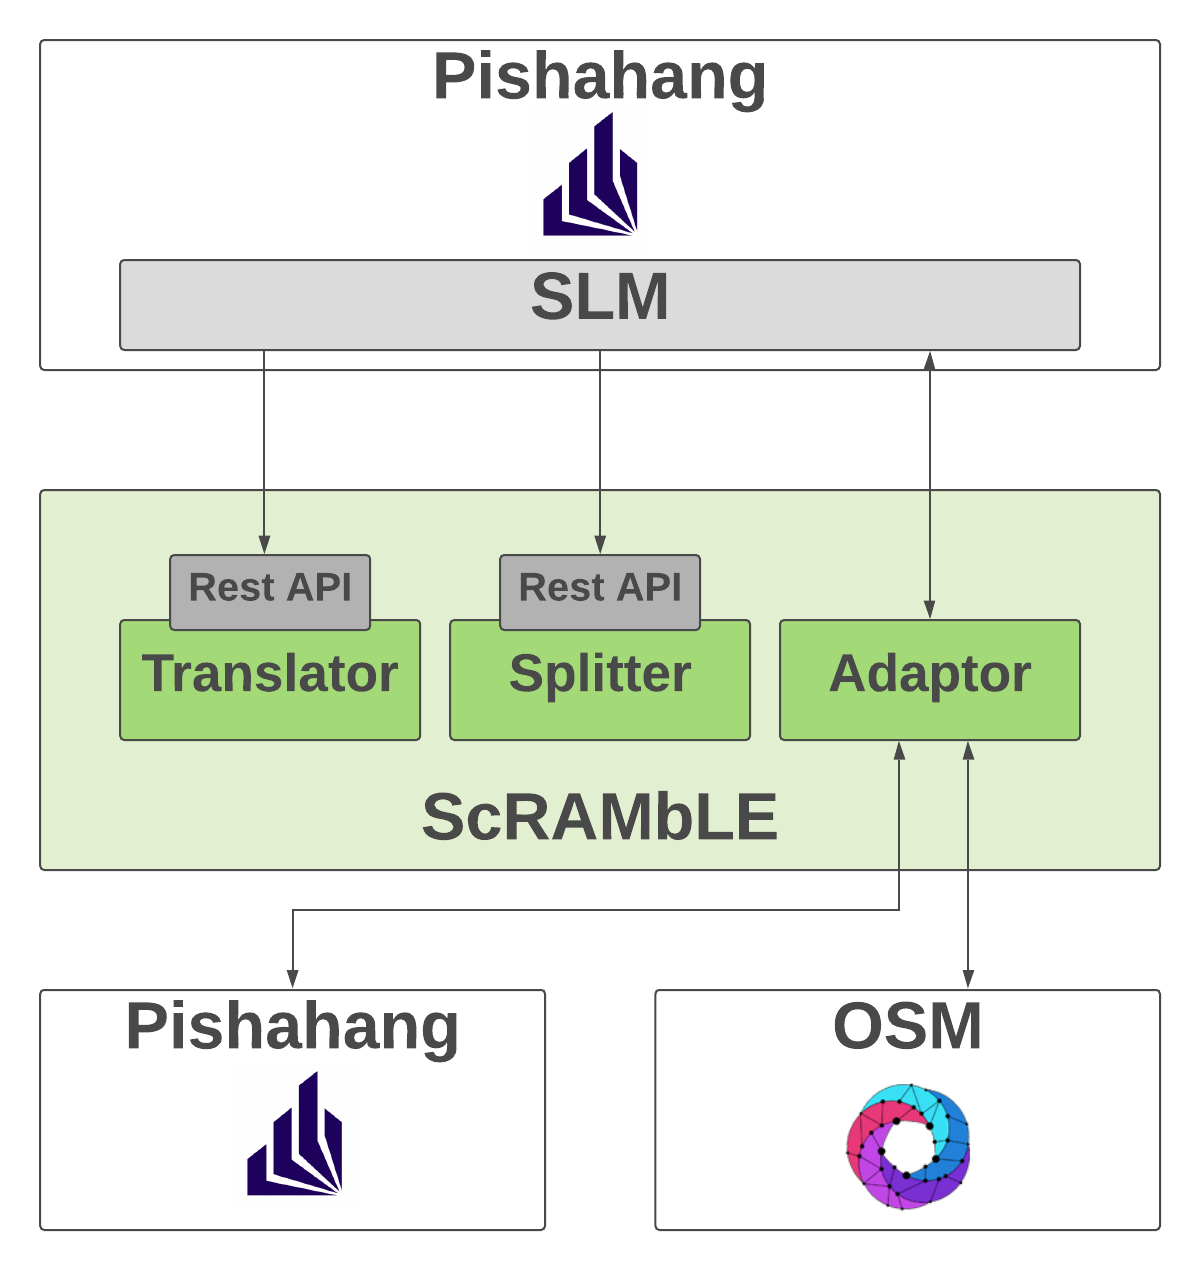
\includegraphics[width=0.9\linewidth]{../figures/ScrambleArchitecture}
	\caption{Scramble Architecture}
	\label{fig:scramble-architecture}
\end{figure}

\begin{figure}[h]
	\centering
	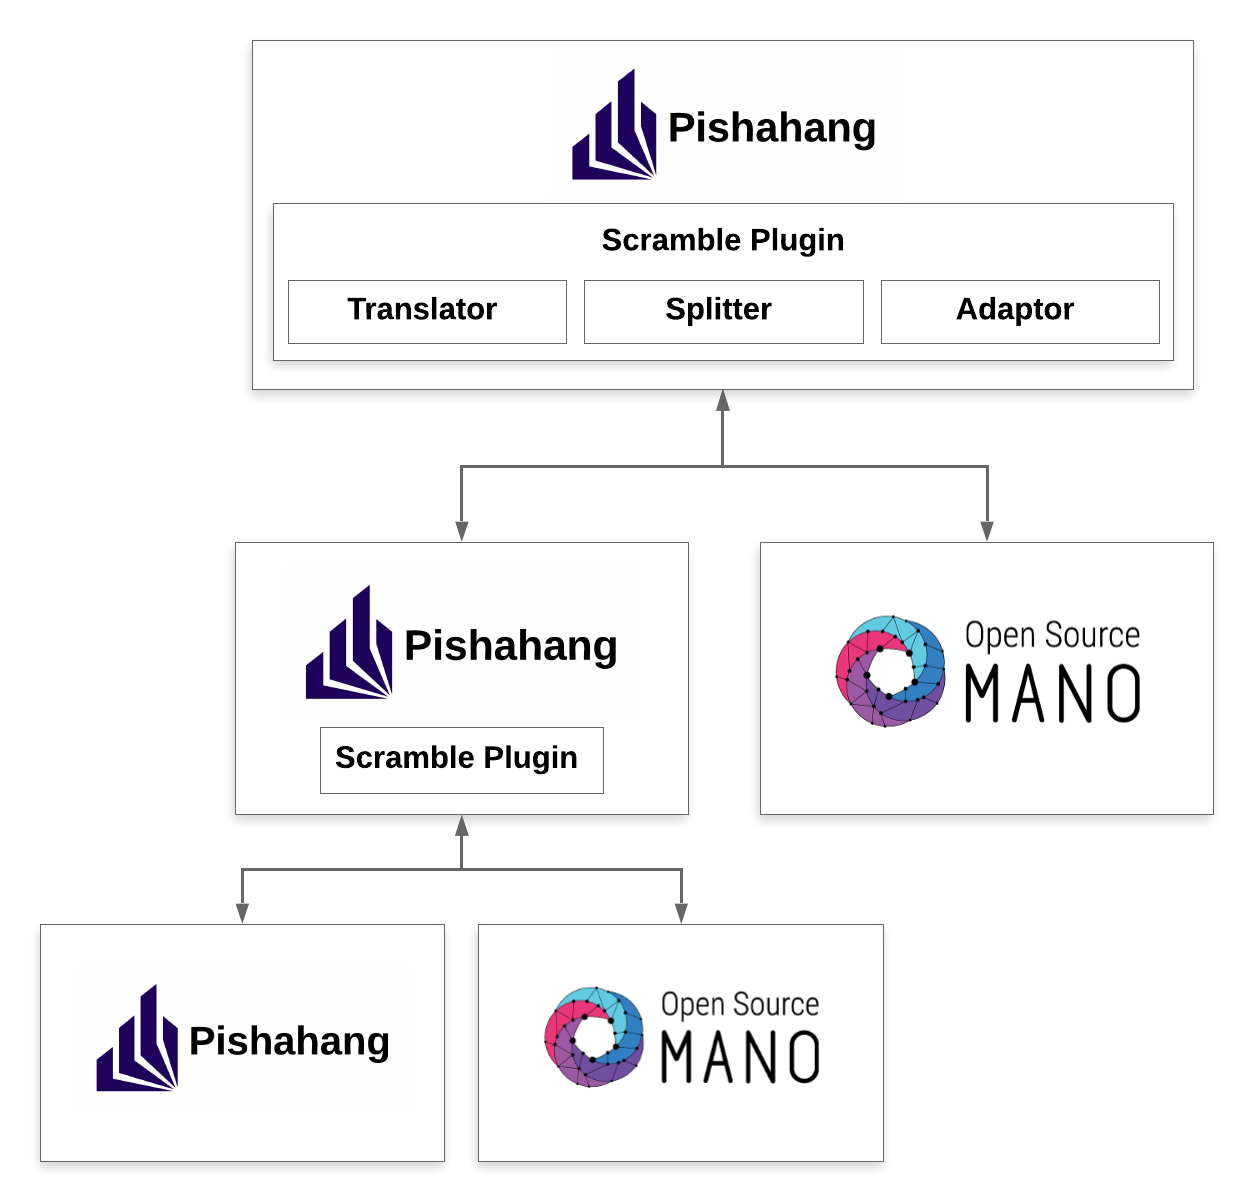
\includegraphics[width=0.9\linewidth]{../figures/ScrambleArch}
	\caption{High-level scramble architecture}
	\label{fig:scramble-arch}
\end{figure}

